% Quick start guide
\documentclass{beamer}

\usetheme {default}

% Title page details
\title {git training}
\subtitle{git, workflows, github}
%\author{latex-beamer.com}
%\institute{KUNBUS GmbH}
%\date{\today}

% Image Logo
\logo{
\includegraphics[width=2.5cm]{kunbus-logo.png}} 

\begin{document}

\begin{frame}
% Print the title page as the first slide
\titlepage
\end{frame}

% Presentation outline
\begin{frame}{Outline}
    \tableofcontents
\end{frame}

\section{What is a VCS?}
\begin{frame}{What is a VCS?}{Version Control System}
\begin{itemize}
	\item Tracks changes
	\item Creates a history over the changes
	\item Provides traceability
	\item Provides attribution
\end{itemize}
\end{frame}

\begin{frame}{Centralized vs. Distributed VCS}{Centralized}
\begin{figure}
	\centering
	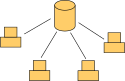
\includegraphics[width=0.7\textwidth]{01_centralized_vcs}
\end{figure}
\end{frame}

\begin{frame}{Centralized vs. Distributed VCS}{Centralized}
\begin{figure}
	\centering
	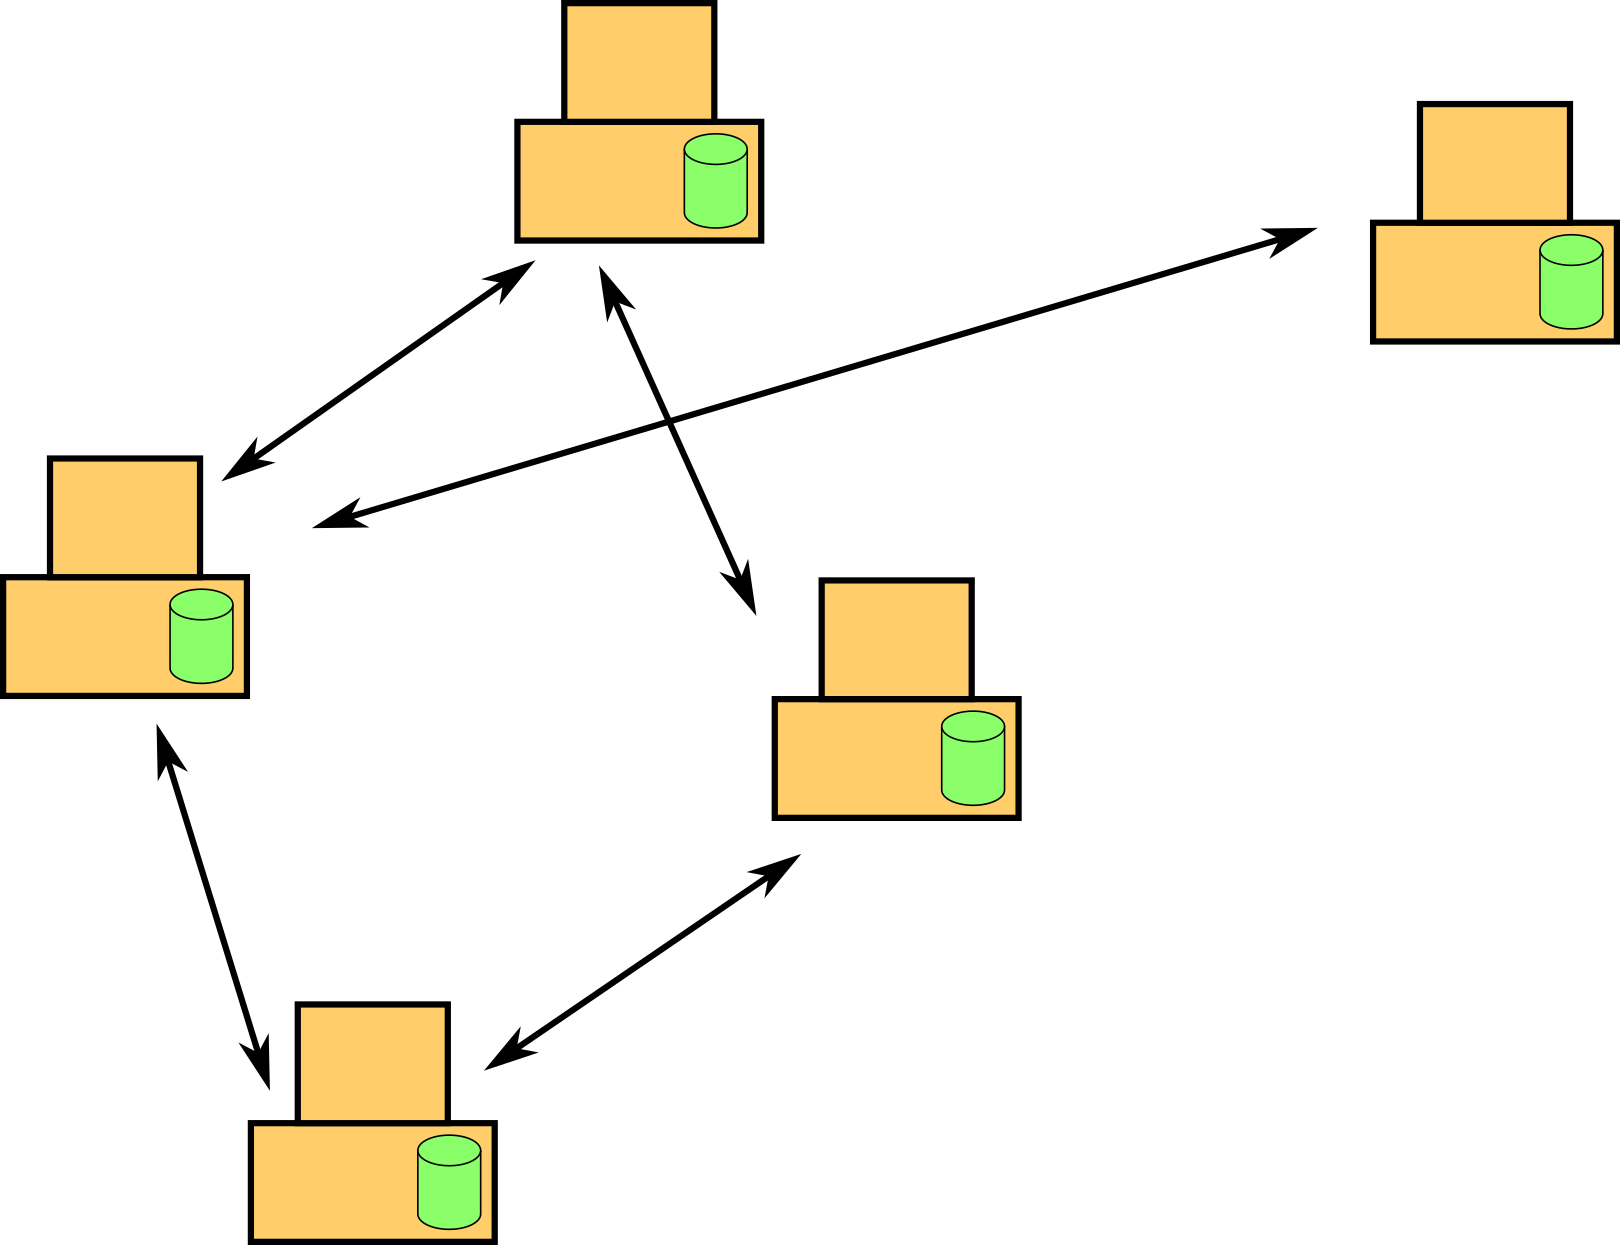
\includegraphics[width=0.7\textwidth]{02_distributed_vcs}
\end{figure}
\end{frame}

\begin{frame}{Deltas vs. Snapshots}{Deltas}
\begin{figure}
	\centering
	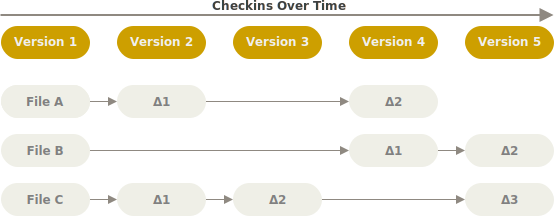
\includegraphics[width=1\textwidth]{deltas}
\end{figure}
\end{frame}

\begin{frame}{Deltas vs. Snapshots}{Snapshots}
\begin{figure}
	\centering
	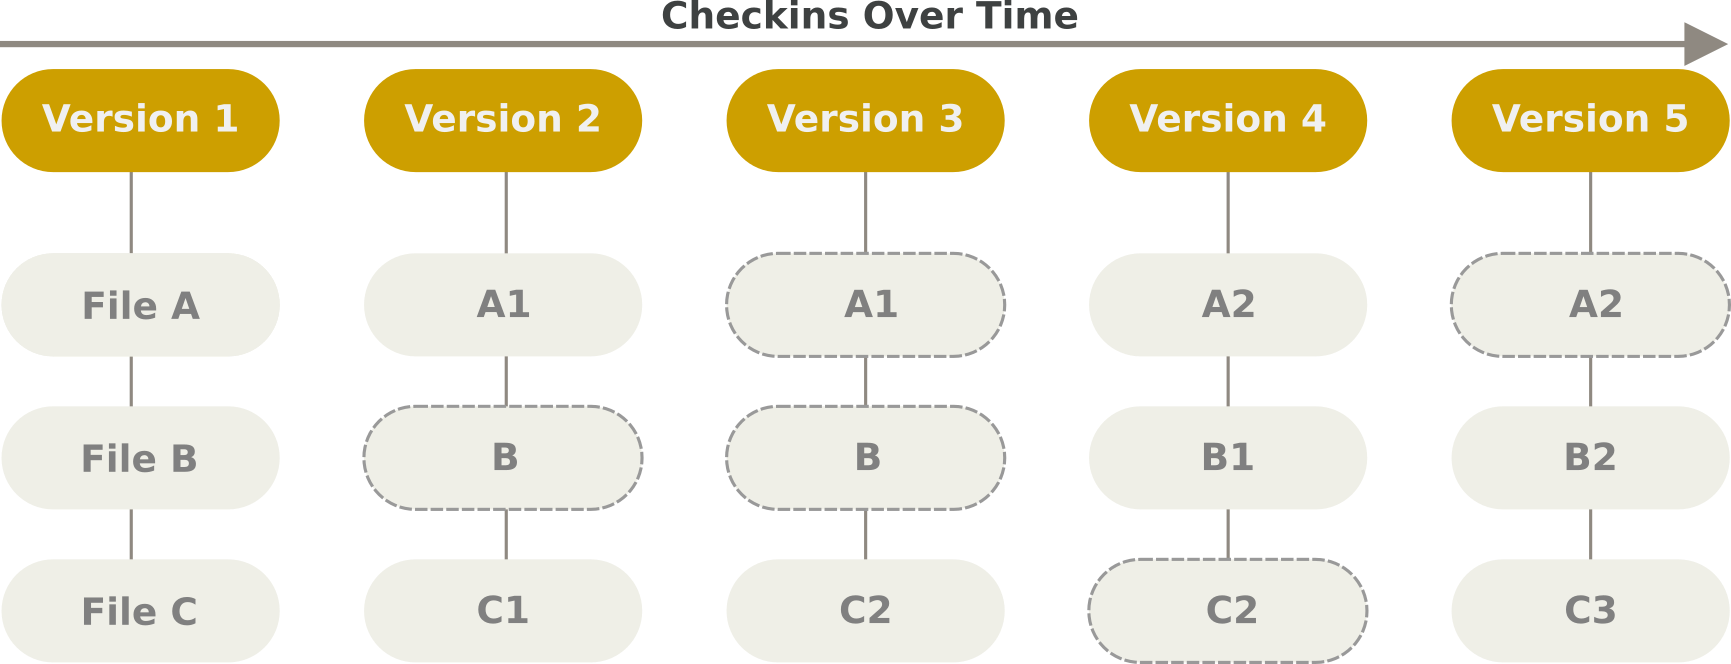
\includegraphics[width=1\textwidth]{snapshots}
\end{figure}
\end{frame}

\end{document}
